\clearpage\thispagestyle{empty}\newgeometry{left=3.5cm,right=3.5cm,top=2cm,bottom=2cm}

\vspace*{\stretch{1}}

\adjustbox{center}{\swrule{1.025\textwidth}{1pt}}

\vspace{-0.5cm}
{\center \normalsize \huge \ccLogo\ \ccAttribution\ \ccShareAlike \par}
\vspace{0.5cm}

Ce document est placé sous licence Creative Commons \myccbysa.

%\begin{wrapfigure}[5]{r}{2cm}\vspace{-0.5cm}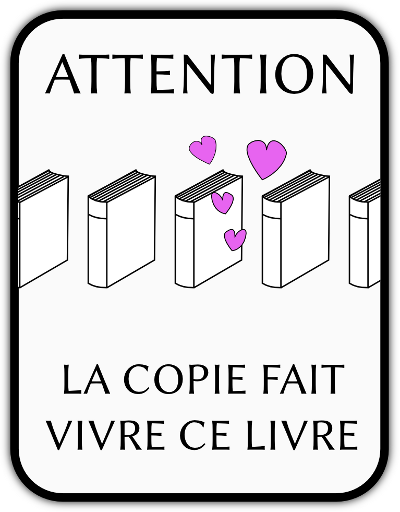
\includegraphics[width=2.1cm]{images/photocopillage.png}\end{wrapfigure}%
La copie, la redistribution, et la modification sont encouragées, sous seules conditions d’attribution de l’auteur et de conservation de cette licence. Le texte intégral de la licence est accessible à l’\textsc{url} \href{https://creativecommons.org/licenses/by-sa/3.0/deed.fr}{https://creativecommons.org/licenses/by-sa/3.0/deed.fr}. L’ouvrage bénéficie d’une contribution de Philippe Depondt (\S\ref{ch_histoire_degre_chaleur_depondt}) sous même licence. Enfin, de nombreuses illustrations d’auteurs divers sous licences compatibles sont intégrées à ce document ; leurs licence et auteur sont indiquées dans chaque cas.

\vspace{0.3cm}
\adjustbox{center}{\swrule{1.025\textwidth}{1pt}}
\vspace{0.1cm}

Ce document est édité par un groupe de travail \textit{Framabook} en vue de sa publication sous forme de livre début 2015. Un wiki de travail est mis à disposition à l’adresse \href{http://dokuwiki.framabook.org/doku.php?id=framabookthermodynamique}{dokuwiki.framabook.org/doku.php?id=framabookthermodynamique}, sur lequel vous pouvez participer à son amélioration. Vous pouvez également envoyer vos retours d’expérience, signalements, critiques et autres, toujours très vivement appréciés, directement à Olivier Cleynen à l’adresse olivier.cleynen\raisebox{-0.2ex}{
\includegraphics[width=1.7ex]{images/arobase.png}}ariadacapo.net.

De nombreuses personnes, en corrigeant des erreurs ou proposant des améliorations, ont réduit l’entropie de ce document, parmi lesquelles : {\small\textit{Antoine\ L., Hamassala David Dicko, Kévin\ R., Florianne\ B., Julien\ D., Anthony Jouny, Thomas\ N., Amazigh.L.H, Victor\ D., Daniel\ C.-N., Pierrick Degardin, Arthur\ A., Ulrick\ M., Solène\ J., Florian Paupert, Gatien Bovyn, Mehdi\ Z., Jean-Bernard Marcon, Luc Benoit, Christophe Masutti, Thibault Mattera, Mireille \textsc{Bernex}}}. L’auteur leur adresse beaucoup de gratitude ! Toutes les erreurs restantes dans le présent document sont le fait d’Olivier Cleynen.

\vspace{0.3cm}
\adjustbox{center}{\swrule{1.025\textwidth}{1pt}}

\vspace*{\stretch{1}}

\restoregeometry
